\section{Memory Management}
\label{sec:mem_management}

\begin{figure*}[]
    \centering
    \setlength{\abovecaptionskip}{0cm}
    % \setlength{\belowcaptionskip}{-0.3cm}
    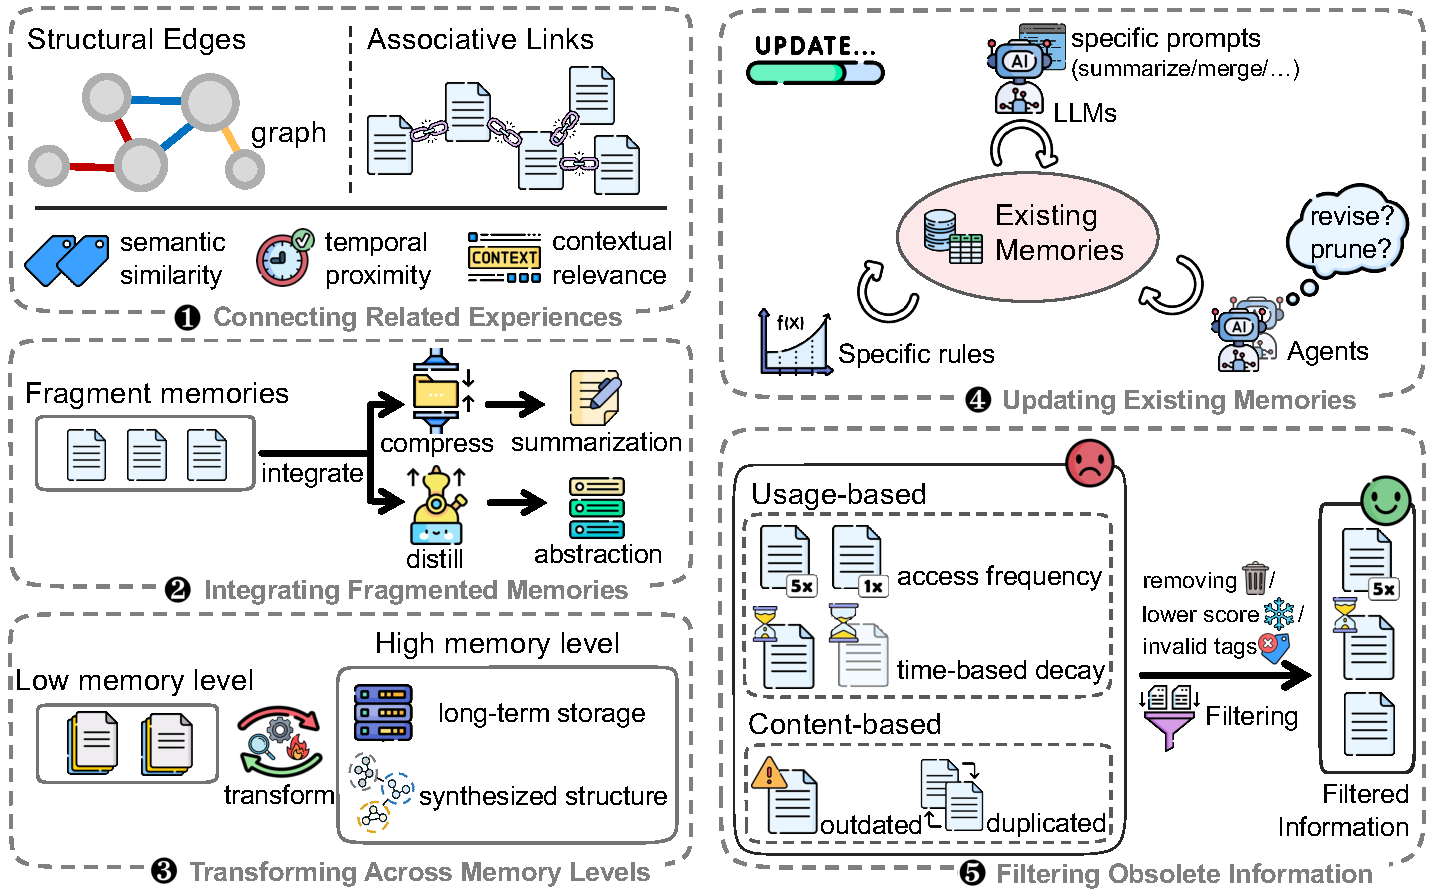
\includegraphics[width=0.82\linewidth]{figures/management.pdf}
    \caption{Workflow of the memory management process.}
    \label{fig:management}
\end{figure*}
%subtitles could be more centralized?

The memory management process governs how an agent system maintains, refines, and evolves its memory over time. 
As illustrated in Figure~\ref{fig:management}, it mirrors the human memory lifecycle, encompassing five core operations: connecting related experiences, integrating fragmented information, transforming short-term into long-term memory, updating outdated content, and filtering obsolete knowledge. 
Table~\ref{tab:management_methods} summarizes how representative agent memory methods instantiate these operations through different implementation paradigms. 
Through this process, the system maintains a coherent, efficient, and adaptive memory state that supports continual learning and reasoning.

\noindent {\Large \ding{182}} \textbf{Connecting Related Experiences.}  
Humans naturally associate related events across time and context; agent systems emulate this through \textit{connection}.  
This mechanism establishes explicit connections between memory entries that share semantic similarity, temporal proximity, or contextual relevance, realized through either \textbf{structural edges} within a graph or \textbf{associative links} across discrete records.
% Systems such as {\tt A-Mem}, {\tt Zep}, and {\tt MemoryOS} leverage associative connections to organize related experiences into structured knowledge representations, enabling reasoning and retrieval across conceptually or temporally aligned memories.
For example, memory methods such as {\tt A-MEM} and {\tt MemoryOS} leverage associative links based on semantic similarity or continuity, enabling synchronous updates and alignment across connected memories. Separately, graph-based methods such as {\tt Zep} and {\tt Mem0$^g$} focus on connecting individual episode or entity nodes to support reasoning and retrieval across conceptually or temporally aligned memories.

\noindent {\Large \ding{183}} \textbf{Integrating Fragmented Memories.}  
Humans tend to summarize daily experiences, retaining only key events while discarding details.  
Agent systems achieve similar \textit{integration} through \textbf{abstraction} or \textbf{summarization}. 
For example, {\tt MemoryBank} aggregates repetitive daily records into event summaries and refines a global user profile as experiences accumulate.  
Likewise, {\tt MemoChat} groups related dialogues under shared topics and produces topic-level summaries.  
This process reduces redundancy, distills essential information, and transforms scattered memories into concise high-level representations suitable for long-term storage.

\noindent {\Large \ding{184}} \textbf{Transforming Across Memory Levels.}  
Human memory gradually transfers important information from low-level to high-level storage, reinforcing what is repeatedly recalled.  
Agent systems adopt similar hierarchical migration mechanisms.  
For instance, {\tt MemoryOS} implements a two-stage migration strategy: short-term memories are first moved to mid-term storage following a First-In, First-Out (FIFO) policy, and mid-term memories are then promoted to long-term storage using a heat-based score that jointly considers access frequency and recency.  
Additionally, memory methods such as {\tt Zep} organize semantically related memories into communities, forming structured, interconnected long-term representations.  
This stage strengthens persistent knowledge while maintaining efficiency.

\noindent {\Large \ding{185}} \textbf{Updating Existing Memories.}  
Humans constantly revise their memories by integrating new experiences and correcting inconsistencies.  
Agent systems follow a similar principle through three main updating paradigms:
(1) \textbf{Rule-based updating}, where existing memories are updated according to predefined rules. For example, {\tt MemoryBank} adopts Ebbinghaus's Forgetting Curve theory to adjust memory strength over time. In {\tt MemoryOS}, new memories are integrated into existing structures based on semantic and keyword similarities;
(2) \textbf{LLM-based updating}, where large language models are prompted to summarize, merge, or resolve conflicts between entries. To give an example, {\tt MemTree} updates its memory by relying on the LLM to execute a specialized Aggregate Operation, where the prompt and the count of descendants guide the LLM to appropriately compress and generalize information before the new content is written back to the parent node. Taking another example, the update process in {\tt Zep} requires the LLM to execute resolution tasks by strictly following detailed semantic constraints and procedural guidelines given in the prompts.
(3) \textbf{Agent-based updating}, where agents autonomously decide which operations (e.g., revise, merge, prune) to apply, as in {\tt MemGPT} and {\tt MemOS}. To be more specific, agents are granted access to current context as well as historical or archival memory entries and learn to utilize specialized system tools for managing memories efficiently and flexibly.
These strategies ensure that memory remains accurate, consistent, and aligned with evolving knowledge.

\noindent {\Large \ding{186}} \textbf{Filtering Obsolete Information.}  
Finally, the memory system must remain compact and relevant by filtering outdated or redundant information, which can be achieved by either directly removing the memories, lowering their assigned weight score, or applying a status label (such as ``invalid''). This \textit{filtering} process parallels human forgetting, which selectively fades unused or irrelevant memories.  
(1) \textbf{Usage-based filtering}, as seen in {\tt MemoryOS} and {\tt MemoryBank}, relies on access frequency and time-based decay. Memories created a long time ago and rarely retrieved are filtered first.  
(2) \textbf{Content-based filtering} examines semantic similarity and leverages LLMs to detect and filter duplicated or outdated knowledge, such as in {\tt Mem0} and {\tt Mem0$^g$}, reducing noise and improving retrieval precision.  
Together, these mechanisms sustain an efficient, lightweight memory that supports ongoing adaptation and learning.


\begin{table*}[]
  \centering
  \caption{Comparison of implementation paradigms for memory management operations; ``N/A'' means that this operation is not explicitly implemented.}
  % \renewcommand{\arraystretch}{1.25}
  \label{tab:management_methods}
  \begin{tabular}{l|c|c|c|c|c}
     \toprule
     \rowcolor{gray!20}
      \textbf{Method} & \textbf{Connecting} & \textbf{Integrating} & \textbf{Transforming} & \textbf{Updating}& \textbf{Filtering} \\
     \midrule
      {\tt A-MEM} & Associative Links & N/A & N/A & LLM-based & N/A \\
      {\tt MemoryBank} & N/A & Summarization & N/A & Rule-based & Usage-based \\
      {\tt MemGPT} & N/A & Summarization & Stage-wise Transfer & Agent-based & N/A \\
      {\tt Mem0} & N/A & Summarization & N/A & Agent-based & Content-based \\
      {\tt Mem0$^g$} & Structural Edges & N/A & N/A & LLM-based & Content-based \\
      {\tt MemoChat} & N/A & Abstraction & N/A & N/A & N/A \\
      {\tt Zep} & Structural Edges & N/A & Community Formation & LLM-based & N/A \\
      {\tt MemTree} & Structural Edges & Summarization & N/A & LLM-based & N/A \\
      {\tt MemoryOS} & Associative Links & Abstraction + Summarization & Stage-wise Transfer & Rule-based & Usage-based \\
      {\tt MemOS} & Structural Edges & Abstraction + Summarization & N/A & Agent-based & N/A \\
     \bottomrule
  \end{tabular}
\end{table*}

% \section{Memory management}
% \label{sec:mem_management}
% Memory management is a crucial component in agent memory systems, encompassing three key operations: consolidating, updating, and filtering. Each operation may be realized using a variety of strategies, which we describe in detail below.


% % \subsection{Consolidating}
% % \label{sec:mem_consolidation}
% % % The \textit{consolidation} substage aims to merge newly extracted memory with existing memory, ensuring coherence and avoiding redundancy.
% % The consolidation substage enhances the coherence, relevance, and utility of the memory system by integrating and reorganizing memory entries into higher-level structures. Analysis of recent memory systems reveals four major consolidation mechanisms:

% % \noindent {\Large \ding{182}} \textbf{Connection.}  

% % Connection denotes the explicit establishment of links between memory entries that exhibit semantic similarity, temporal proximity, or shared interaction context, which can be found in methods like A-mem, Zep and MemOS. This mechanism facilitates the discovery and retrieval of related information, which provides a richer contextual background for reasoning and decision-making. 

% % \noindent {\Large \ding{183}} \textbf{Abstracting.}  
% % % Abstracting involves generating high-level summaries or compact representations from detailed or fragmented memories. This often leverages LLMs for summarization or user portrait generation. Abstraction reduces redundancy and distills essential information for efficient retrieval and downstream tasks.
% % Abstracting involves generating high-level summaries or compact representations from detailed or fragmented memorie, which often leverages LLMs for summarization or user portrait generation. In Memorybank, daily events with the same timestamps are combined into event summaries and a global user portrait is continuously maintained and refined as events accumulate. In MemoChat, related dialogues are grouped under the same topic, and a corresponding topic summary is generated. Abstraction reduces redundancy and distills essential information for efficient retrieval and downstream tasks.

% % \noindent {\Large \ding{184}} \textbf{Unification.} 
% % Unification consolidates heterogeneous memory types into a unified data structure, such as MemCube. Specifically, MemCube integrates plaintext memory(external, editable knowledge), activation memory(transient runtime states such as KV-cache), and parameter memory (internalized long-term knowledge) within a common schema.  By standardizing representation, memory systems can process different kinds of memories in a consistent manner, which can, to a large extent, smooth memory operations and simplify management.

% % \noindent {\Large \ding{185}} \textbf{Community identification.} 
% % Community identification means discovering and organizing groups of memories. This is usually achieved by identifying and clustering memories or entities that are similar topics or are strongly connected. \textit{Zep} serves as a representative example, as it clusters semantically related memories into communities to facilitate efficient retrieval and contextual understanding. By grouping relevant memories together, community identification helps access related information and discover patterns among topics efficiently.


% % \subsection{Updating}
% % \label{sec:mem_updating}
% % The \textit{updating} operation mimics the human process of memory revision, integrating new experiences, adjusting inconsistent information, and reinforcing salient knowledge, to maintain a coherent and up-to-date memory state.
% % Specifically, there are three memory updating strategies in the existing agent memory systems.

% % \noindent {\Large \ding{182}} \textbf{Rule-based updating.} Memory is updated based on a set of {\it manually predefined rules} that determine when and how modifications occur.
% % For example, {\tt MemoryOS} employs a two-stage memory migration strategy.
% % In the first stage, short-term memories are transferred to mid-term storage following a First-In, First-Out (FIFO) policy.
% % In the second stage, mid-term memories are promoted to long-term storage according to a heat-based scoring mechanism that jointly accounts for access frequency and the time elapsed since the most recent retrieval.
% % This design mirrors the human memory mechanism, where the brain selectively retains important information while discarding less relevant details.
% % Another example is MemoryBank, which adopts an updating mechanism inspired by the Ebbinghaus forgetting curve~\cite{}.
% % Each memory entry is associated with a score that decays exponentially over time and is reinforced when recalled.
% % This design enables less relevant or infrequently accessed memories to fade naturally, while frequently recalled information remains longer, resulting in more human-like memory dynamics.


% % \noindent {\Large \ding{183}} \textbf{LLM-based updating.}  This strategy also based on the maully defined xx, prompting LLM to update the memory.

% % Guideline-driven updating refers to approaches in which the memory management process is primarily governed by explicit operational guidelines provided within the prompt. In this framework, the LLM acts according to detailed instructions that specify how to handle each memory management task, such as summarizing content, resolving conflicts between new and existing entries, or identifying communities. The main advantages of guideline-based updating are its consistency and transparency. By following explicit instructions, the LLM’s behavior is predictable and easier to audit, and domain-specific requirements can be easily incorporated through prompt design. A main limitation of guideline-based updating is its strong dependence on prompt engineering. The quality and effectiveness of memory management rely heavily on how well guidelines are designed and articulated. Incomplete or ambiguous instructions can easily lead to mistakes or unexpected behavior, and adapting to new scenarios often requires manual revision of prompts. For instance, fact and node resolution modules in systems like Zep guide the LLM through step-by-step prompts to decide whether a new edge or node duplicates existing ones. Each step explicitly instructs the model to compare semantics, check factual equivalence, and return fields such as $isduplicate$ and matching uuid. To give another example, in MemTree, each node update is guided by prompt rules that adjust the aggregation level based on the number of child nodes—providing either more detailed or more concise summaries accordingly.

% % \noindent {\Large \ding{184}} \textbf{Agent-based Updating.}  
% % Agent-based updating refers to strategies in which an agent, typically a large language model, is granted access to both current and historical memory entries as well as relevant memory management tools. The agent can retrieve and analyze past memories, assess the present context, and independently decide the most suitable operation for each memory entry. This autonomous decision-making process allows the agent to maintain the integrity and freshness of the memory system in a dynamic and complex environment. For example, systems like MemGPT or MEMOS provide the agent system with a set of specialized tools and guidance on how to use them, leaving the agent to autonomously decide which tools to invoke and what operations to perform on memory entries. Similarly, frameworks such as AMem provide the agent with evolution rules for memory updates, allowing it to autonomously decide operations such as "strengthen", "merge", or "prune" to update memory context, neighbours and tags flexibly and effectively. Mem0 likewise grants the LLM freedom to decide what operations to perform on memories.




% % \subsection{Filtering}
% % \label{sec:mem_filtering}
% % The filtering substage is responsible for removing outdated, redundant, or low-value memories to maintain the efficiency and relevance of the memory system. Based on the analysis of recent memory architectures, filtering mechanisms can be broadly divided into the following two categories:

% % \noindent {\Large \ding{182}} \textbf{Usage-based Filtering.}  
% % Usage-based filtering relies on temporal and frequency-based metrics to determine which memories should be forgotten. Each memory entry is evaluated by considering factors such as age the the number of times it has been accessed. Entries that have remained unused for extended periods or have low access frequencies are more likely to be removed. 

% % \noindent {\Large \ding{183}} \textbf{Content-based Filtering.}  
% % Content-based filtering examines the substance of memory entries to decide whether a memory is redundant. Identifying and eliminating memories that are redundant is often implemented through designed algorithms or with the assistance of large language models.

% % \subsection{Enhancement}
% % \label{sec:mem_enhancement}
% % The enhancement substage is used to make important memories easier to identify and use. It includes mechanisms that mark, place, or display core memories in ways that improve their visibility and availability for later tasks. Here are the three main approaches used by recent memory systems.

% % \noindent {\Large \ding{182}} \textbf{Tagging.}  
% % Tagging means adding an explicit label or marker to a memory entry to show its importance. For instance, MemoryOS uses heat values, where higher heat scores mean the corresponding memories are more important. These kind of priority labels help the memory system rank and select key memories.

% % \noindent {\Large \ding{183}} \textbf{Prominent positioning.} 
% % Prominent positioning arranges important memories so that they are stored in high-priority areas of the memory system. For instance, MemGPT places core memories in the main contenxt window and MemOS put most frequently used or most important
% % memories in a parametric memory pool. 

% % \noindent {\Large \ding{184}} \textbf{Key information surfacing.} 
% % key information surfacing extracts the main topics or key terms from important memories and displays them in visible places such as community names. This allows the memory system to have access to key information without visiting memory entries.

% \subsection{Consolidating}
% \label{sec:mem_merging}

% The \textit{consolidating} operation focuses on integrating fragmented or short-term memories into coherent and stable long-term representations. 
% It mirrors the human cognitive process of memory consolidation, where transient experiences are gradually fused into durable knowledge through association, abstraction, and reinforcement. 
% In agent systems, consolidation governs the transformation from short-term memory (STM) to long-term memory (LTM) by merging semantically or temporally related experiences into structured, higher-level representations. 
% This operation enhances the system’s coherence, persistence, and retrieval efficiency by building long-term organization rather than altering existing content.

% \noindent {\Large \ding{182}} \textbf{Connection.}
% Connection establishes explicit links between memory entries that share semantic similarity, temporal proximity, or contextual relevance. 
% Systems such as {\tt A-Mem}, {\tt Zep}, and {\tt MemoryOS} exemplify this mechanism by forming associative networks that link related events or topics. 
% Such interconnections enable richer contextual graphs, facilitating reasoning and cross-referencing across related experiences.

% \noindent {\Large \ding{183}} \textbf{提炼.}
% 提炼 generates concise, high-level summaries or representations from detailed or repetitive memories. 
% For instance, {\tt MemoryBank} aggregates daily events with identical timestamps into event summaries and continuously refines a global user portrait as experiences accumulate. 
% Similarly, {\tt MemoChat} groups related dialogues under shared topics and produces topic-level summaries. 
% This process reduces redundancy, distills essential information, and yields compact long-term memory units suitable for efficient retrieval and reasoning.

% \noindent {\Large \ding{184}} \textbf{.}
% 短期转换到长期，社区、
% Community identification organizes related memories into cohesive clusters or communities based on semantic or relational similarity. 
% For example, {\tt Zep} identifies and clusters strongly connected entities into topical communities, forming an intermediate layer between raw episodic data and abstract knowledge. 
% This mechanism captures high-level patterns, promotes efficient retrieval, and reflects how human memory organizes experiences into interconnected conceptual structures.
% 把MemoryOS根据那个转换FIFO长短期记忆的也放这里

% \subsection{Updating}
% \label{sec:mem_updating}

% The \textit{updating} operation emulates the human process of memory revision—integrating new experiences, correcting inconsistencies, and reinforcing important knowledge to maintain a coherent and up-to-date memory state. 
% While consolidation aims to organize and stabilize long-term knowledge, updating operates at a finer granularity, directly modifying individual memory entries to reflect the most current and accurate information. 
% Existing systems generally implement three primary updating paradigms.

% \noindent {\Large \ding{182}} \textbf{Rule-based Updating.}
% In rule-based strategies, memory is updated according to a set of predefined heuristics that determine when and how modifications occur. 
% For example, {\tt MemoryOS} employs a two-stage migration mechanism: short-term memories are first transferred to mid-term storage using a First-In, First-Out (FIFO) policy, and mid-term memories are then promoted to long-term storage based on a heat-based score that considers both access frequency and recency. 
% This design reflects the human tendency to reinforce frequently recalled information while allowing less relevant details to fade. 
% Similarly, {\tt MemoryBank} adopts an updating mechanism inspired by the Ebbinghaus forgetting curve~\cite{}, where each memory entry’s strength decays exponentially over time and is reinforced upon recall, yielding more human-like retention dynamics.

% \noindent {\Large \ding{183}} \textbf{LLM-based Updating.}
% LLM-based updating employs prompt-guided instructions to direct large language models in performing specific modifications such as summarization, conflict resolution, or information merging. 
% For example, {\tt Zep} uses step-by-step prompt templates that instruct the model to assess semantic equivalence and determine whether new information duplicates existing nodes or edges. 
% Likewise, {\tt MemTree} adjusts node abstraction levels based on structural cues, dynamically controlling the granularity of retained information. 
% This paradigm offers semantic flexibility and interpretability but remains sensitive to the completeness and clarity of prompt design.

% \noindent {\Large \ding{184}} \textbf{Agent-based Updating.}
% Agent-based updating grants the LLM autonomous decision-making capabilities to retrieve, analyze, and revise memories based on the current context and historical information. 
% Systems such as {\tt MemGPT} and {\tt MEMOS} equip agents with specialized memory management tools, enabling them to autonomously determine which operations (e.g., revise, merge, prune) to apply. 
% {\tt AMem} further defines adaptive evolution rules—such as \textit{strengthen}, \textit{merge}, and \textit{prune}—allowing the agent to flexibly update contextual relationships and semantic tags. 
% This approach enhances adaptivity and intelligence but requires supervision to ensure stability and prevent semantic drift.

% \subsection{Filtering}

% \label{sec:mem_filtering}

% The \textit{filtering} operation is designed to maintain the efficiency, compactness, and relevance of the memory system by pruning redundant, outdated, or low-value entries.
% It mirrors the human forgetting process, which selectively removes less significant experiences while retaining essential ones.
% Filtering acts as the final stage in the memory lifecycle, following merging and updating, to ensure the memory space remains both lightweight and focused.

% \noindent {\Large \ding{182}} \textbf{Usage-based Filtering.}
% Usage-based filtering evaluates memory entries based on their temporal and access-frequency characteristics.
% Entries that have not been retrieved for extended periods or that exhibit low engagement scores are more likely to be removed.
% This principle, adopted by systems such as {\tt MemoryOS}, reflects human forgetting driven by disuse — information that is rarely recalled gradually fades from memory.

% \noindent {\Large \ding{183}} \textbf{Content-based Filtering.}
% Content-based filtering examines the semantic substance of stored memories to identify redundancy or obsolescence.
% Algorithmic similarity checks or LLM-based semantic comparisons are often employed to detect overlapping or outdated entries.
% By pruning such low-value memories, the system reduces noise, preserves factual consistency, and improves retrieval precision.








